%%%%%%%%%%%%%%%%%%%%%%%%%%%%%%%%%%%%%%%%%
% Beamer Presentation
% LaTeX Template
% Version 1.0 (10/11/12)
%
% This template has been downloaded from:
% http://www.LaTeXTemplates.com
%
% License:
% CC BY-NC-SA 3.0 (http://creativecommons.org/licenses/by-nc-sa/3.0/)
%
%%%%%%%%%%%%%%%%%%%%%%%%%%%%%%%%%%%%%%%%%

%----------------------------------------------------------------------------------------
%	PACKAGES AND THEMES
%----------------------------------------------------------------------------------------

\documentclass{beamer}

\mode<presentation> {

% The Beamer class comes with a number of default slide themes
% which change the colors and layouts of slides. Below this is a list
% of all the themes, uncomment each in turn to see what they look like.

%\usetheme{default}
%\usetheme{AnnArbor}
%\usetheme{Antibes}
%\usetheme{Bergen}
%\usetheme{Berkeley}
%\usetheme{Berlin}
%\usetheme{Boadilla}
%\usetheme{CambridgeUS}
%\usetheme{Copenhagen}
%\usetheme{Darmstadt}
%\usetheme{Dresden}
%\usetheme{Frankfurt}
%\usetheme{Goettingen}
%\usetheme{Hannover}
%\usetheme{Ilmenau}
%\usetheme{JuanLesPins}
%\usetheme{Luebeck}
\usetheme{Madrid}
%\usetheme{Malmoe}
%\usetheme{Marburg}
%\usetheme{Montpellier}
%\usetheme{PaloAlto}
%\usetheme{Pittsburgh}
%\usetheme{Rochester}
%\usetheme{Singapore}
%\usetheme{Szeged}
%\usetheme{Warsaw}

% As well as themes, the Beamer class has a number of color themes
% for any slide theme. Uncomment each of these in turn to see how it
% changes the colors of your current slide theme.

%\usecolortheme{albatross}
%\usecolortheme{beaver}
%\usecolortheme{beetle}
%\usecolortheme{crane}
%\usecolortheme{dolphin}
%\usecolortheme{dove}
%\usecolortheme{fly}
%\usecolortheme{lily}
%\usecolortheme{orchid}
%\usecolortheme{rose}
%\usecolortheme{seagull}
%\usecolortheme{seahorse}
%\usecolortheme{whale}
%\usecolortheme{wolverine}

%\setbeamertemplate{footline} % To remove the footer line in all slides uncomment this line
%\setbeamertemplate{footline}[page number] % To replace the footer line in all slides with a simple slide count uncomment this line

%\setbeamertemplate{navigation symbols}{} % To remove the navigation symbols from the bottom of all slides uncomment this line
}

\usepackage{graphicx} % Allows including images
\usepackage{changepage}
\usepackage{amsmath}
\usepackage{booktabs} % Allows the use of \toprule, \midrule and \bottomrule in tables
\usepackage{xcolor}
\usepackage{listings} % for syntax highlighting
\usepackage{multicol}
\lstloadlanguages{Ruby}
\lstloadlanguages{C++}
\graphicspath{{./images/}}

%----------------------------------------------------------------------------------------
%	TITLE PAGE
%----------------------------------------------------------------------------------------

\title[Intro to C++20]{Introduction to C++20} % The short title appears at the bottom of every slide, the full title is only on the title page

\author{Raleigh Littles} % Your name
\institute[Karl Storz Imaging] % Your institution as it will appear on the bottom of every slide, may be shorthand to save space
{
 \\ % Your institution for the title page
\medskip
\textit{} % Your email address
}
\date{\today} % Date, can be changed to a custom date
\begin{document}

\begin{frame}
\titlepage % Print the title page as the first slide
\end{frame}

\begin{frame}
\frametitle{Overview} % Table of contents slide, comment this block out to remove it
\tableofcontents % Throughout your presentation, if you choose to use \section{} and \subsection{} commands, these will automatically be printed on this slide as an overview of your presentation
\end{frame}

%----------------------------------------------------------------------------------------
%	PRESENTATION SLIDES
%----------------------------------------------------------------------------------------

%------------------------------------------------
\section{Timeline} % Sections can be created in order to organize your presentation into discrete blocks, all sections and subsections are automatically printed in the table of contents as an overview of the talk
%------------------------------------------------

% Get rid of the section below
%\section{Subsection Example} % A subsection can be created just before a set of slides with a common theme to further break down your presentation into chunks

\begin{frame}
\frametitle{Current timeline of modern C++}

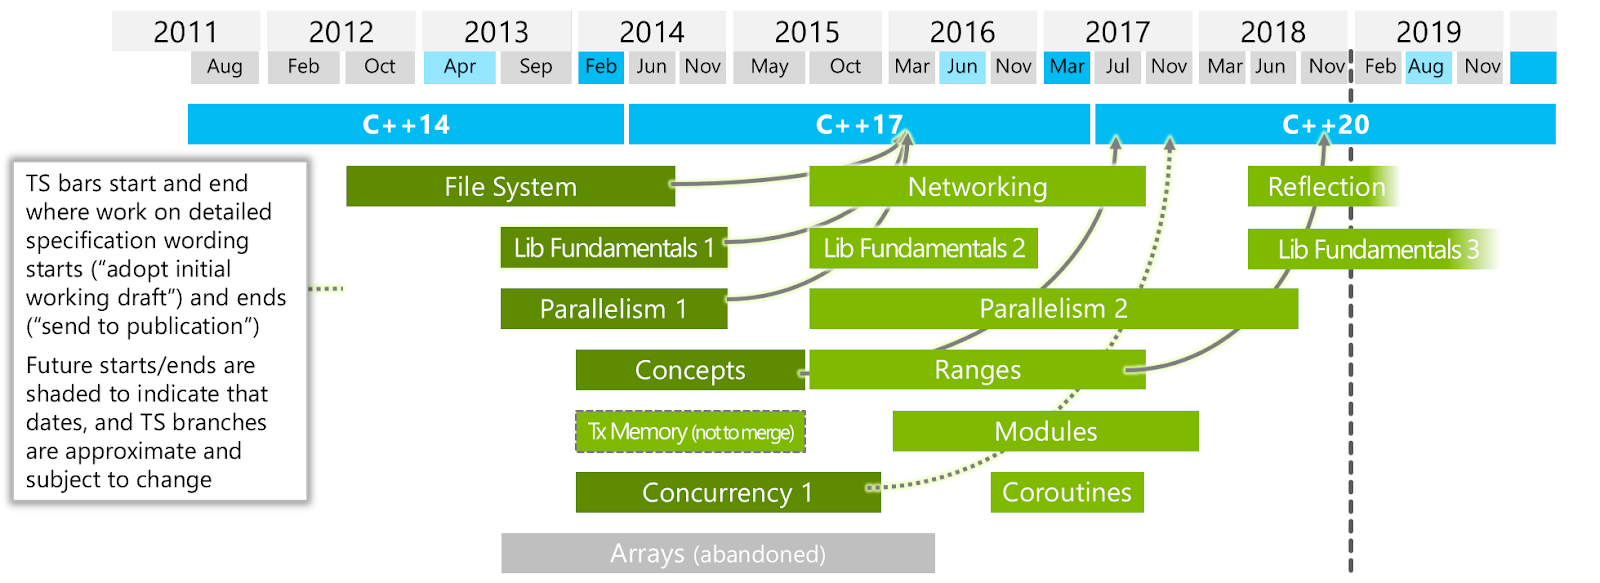
\includegraphics[width=\textwidth,height=\textheight,keepaspectratio]{timeline}

\vspace{1em}

From: https://isocpp.org/std/status

\end{frame}

%------------------------------------------------

\begin{frame}
\frametitle{C++ committee works asynchronously}
\begin{itemize} \setlength\itemsep{2 em} % double space for itemize
\item C++ committee votes on certain features, received from proposals
\item These features, once voted on, go into the C++ standard
\item Particularly large/challenging modules (?) are deferred to be \emph{technical standards}
\item Technical standards are worked on independently and can be delivered later (even once the standard itself is finished!)
\end{itemize}
\end{frame}

%------------------------------------------------

\begin{frame}
\frametitle{Current commitee progress}
{ 
\setbeamercolor{block title}{bg=red!100}
\begin{block}{Meeting \#1: July 2017}
Voted in: \underline{Concepts}, designated initializers, new lambda capture syntax, template parameter lists, ...
\end{block}

\begin{block}{Meeting \#2: November 2017}
Voted in: variable initialization on ranged-for statements, bit-casting object representations, \underline{three-way comparison operator}, \underline{atomic shared pointers}, ...
\end{block}

\begin{block}{Meeting \#3: June 2018}
Voted in: \underline{Contracts}, feature test macros, \underline{Ranges}, explicit booleans, \texttt{constexpr} virtual functions
\end{block}

\begin{block}{Meeting \#4: November 2018}
Voted in: \texttt{consteval} keyword, \texttt{constexpr} try-catch, \texttt{constexpr} dynamic casts, \texttt{pointer\_traits}, ...
\end{block}
}
\end{frame}

\begin{frame}
\frametitle{Remaining progress}
{ % Use this to temporarily change the color of a block
\setbeamercolor{block title}{bg=red!30}
\begin{block}{Meeting \#5: Q1 2019}
Last meeting to vote on new features.
Begin drafting C++20 standard. 
\end{block}

\begin{block}{Meeting \#6: Q2 2019}
C++20 internal draft completed, committee begins vote to approve.
\end{block}
}
\end{frame}

%------------------------------------------------

\section{Concepts}

\begin{frame}[fragile]
\frametitle{Concepts: Introduction}
\begin{itemize}
\item "A description of supported operations on a type"
\item Also known as \emph{constraints} -- can you guess why?
\end{itemize}

\lstset{language=C++,
                basicstyle=\ttfamily,
                numbers=left,
		stepnumber=1,
		firstnumber=1,
		xleftmargin=2em,
		frame=single,
		framexleftmargin=1.5em,
		numberfirstline=true,
                keywordstyle=\color{blue}\ttfamily,
                stringstyle=\color{red}\ttfamily,
                commentstyle=\color{green}\ttfamily,
                morecomment=[l][\color{magenta}]{\#}
}
\begin{lstlisting}
    template <class Type>
    concept bool EqualityComparable() 
    {
    	return requires(Type a, Type b) 
    	{
    		{a == b} -> Boolean;
    		{a != b} -> Boolean; 
    	}; 
    }
 
\end{lstlisting}
\end{frame}


\begin{frame}[fragile]
\frametitle{Concepts continued}
\lstset{language=C++,
		numbers=left,
		stepnumber=1,
		firstnumber=1,
		xleftmargin=2em,
		frame=single,
		framexleftmargin=1.5em,
		numberfirstline=true,
                basicstyle=\fontsize{9}{10}\ttfamily,
                keywordstyle=\color{blue}\ttfamily,
                stringstyle=\color{red}\ttfamily,
                commentstyle=\color{green}\ttfamily,
                morecomment=[l][\color{magenta}]{\#}
}
\begin{lstlisting}
    template <class Type>
    concept bool GenericConcept() 
    {
    	return requires(Type a, Type b) 
    	{
    		{OPERATION} -> TYPE;
    	}; 
    }
 
\end{lstlisting}
        
        %Content
        \begin{itemize}
        \item \textit{Does the operation make sense on this template type?} \textit{Are the results convertible to a type that satisfies what you told me to expect?}
        \item \textsl{EqualityComparable} (previous slide) is a \emph{concept}, as well as \textsl{TriviallyCopyable} or \textsl{ReversibleContainer}
        \end{itemize}
\end{frame}


\begin{frame}
\frametitle{Concepts: Benefits}

\begin{itemize}
 \setlength\itemsep{2em}
\item Allows you to specify \emph{interoperability} between templates, à la template interfaces ..
\item .. whereas interfaces are run-time polymorphism, concepts provide \textbf{automatic compile-time} polymorphism
\item Introducing type-checking to template programming makes it \textit{simpler}
\end{itemize}

\end{frame}


\section{Ranges}
\begin{frame}[fragile]
\frametitle{Ranges}
\begin{itemize}
\item Adds range comprehensions, function composition, and lazy evaluation
\item Existing STL containers are being upgraded to ranges
\end{itemize}

\lstset{language=C++,
                basicstyle=\fontsize{9}{10}\ttfamily,
                keywordstyle=\color{blue}\ttfamily,
                stringstyle=\color{red}\ttfamily,
                commentstyle=\color{green}\ttfamily,
                morecomment=[l][\color{magenta}]{\#}
}
\begin{lstlisting}
    std::vector<int> vector{1,2,3};
    
    // C++11
    std::sort(vector.begin(), vector.end());
    
    // C++20
    std::sort(vector);
\end{lstlisting}

\vspace{2em}
Don't let the above example betray you

\end{frame}

%------------------------------------------------

\begin{frame}[fragile]
\frametitle{Ranges: function composition example}

Here's what it looks like in two languages that got Ranges right.

\vspace{2em}

\fbox {
	\parbox{0.9\textwidth}{
	Problem: Find all square numbers under 1000 that are also odd.
	}
	}

\vspace{1em}

\lstset{
                basicstyle=\fontsize{9}{10}\ttfamily,
                keywordstyle=\color{orange}\ttfamily,
                stringstyle=\color{red}\ttfamily,
                commentstyle=\color{green}\ttfamily,
                morecomment=[l][\color{magenta}]{\#}
}
\begin{lstlisting}[language=Ruby]
# Ruby
(1..1000).map{|n| n * n}.select{|i| i.odd? && (1000  > i)}
\end{lstlisting}

\begin{lstlisting}[language=Haskell]
--Haskell
takeWhile(<1000) . filter odd . map(^2)
\end{lstlisting}

\vspace{2em}
\fbox{ 
\texttt{1,9,25,49,81,121,169,225,289,361,441,529,625,729,841,961}
}
\end{frame}


%------------------------------------------------

\begin{frame}[fragile] % Need to use the fragile option when verbatim is used in the slide
% http://modernescpp.com/index.php/the-new-ranges-library
\frametitle{Ranges: function composition example}

\vspace{3em}

\lstset{language=C++,
		numbers=left,
		stepnumber=1,
		firstnumber=1,
		xleftmargin=2em,
		frame=single,
		framexleftmargin=2em,
		numberfirstline=true,
		breakatwhitespace=true,
                basicstyle=\fontsize{9}{10}\ttfamily,
                keywordstyle=\color{blue}\ttfamily,
                stringstyle=\color{red}\ttfamily,
                commentstyle=\color{green}\ttfamily,
                morecomment=[l][\color{magenta}]{\#}
}
\begin{lstlisting}
    #include <ranges>
    
    using namespace std;    
    
    auto odds = ranges::view::transform(
     	[](int i){return i*i; } ) |
     	[](int i){return i % 2 == 0; } ) |
     	[](int i){return i < 1000; } );
    									
    auto oddNumbers = ranges::view::ints(1) | odds;
\end{lstlisting}

\vspace{1em}

Where have we seen this kind of syntax?

\hspace{10em}  
\includegraphics[scale=0.2]{tux.png}
\end{frame}

%------------------------------------------------

\begin{frame}
\frametitle{Perfect squares example explained}
\begin{itemize}
 \setlength\itemsep{2em}
\item The pipe "\textbar " character allows us to \emph{compose} functions on a range
\item View adapters give us a "peek" into a subsection of a range and define the iteration behavior. Don't confuse this with \texttt{string\_view}!
\item Our C++ example used lazy evaluation and we didn't even notice, which is good
\end{itemize}
\end{frame}

%------------------------------------------------

\begin{frame}[fragile] % Need to use the fragile option when verbatim is used in the slide
\frametitle{Perfect squares example review}

\begin{itemize}
\item \texttt{odds} is an example of a view adapter - specifically the \textit{transform} one (others include \textit{filter})
\item \texttt{oddNumbers} takes an infinite sequence of integers (starting with 1) and applies our view adapter to it
\item To print the contents, use any for loop you like, or the new \texttt{ranges::for\_each} for loop 
\end{itemize}

\lstset{language=C++,
		numbers=left,
		stepnumber=1,
		firstnumber=1,
		xleftmargin=2em,
		frame=single,
		framexleftmargin=2em,
		numberfirstline=true,
		breakatwhitespace=true,
                basicstyle=\fontsize{8}{9}\ttfamily,
                keywordstyle=\color{blue}\ttfamily,
                stringstyle=\color{red}\ttfamily,
                commentstyle=\color{green}\ttfamily,
                morecomment=[l][\color{magenta}]{\#}
}
\begin{lstlisting}
    #include <ranges>
    
    using namespace std;    
    
    auto odds = ranges::view::transform(
     	[](int i){return i*i; } ) |
     	[](int i){return i % 2 == 0; } ) |
     	[](int i){return i < 1000; } );
    									
    auto oddNumbers = ranges::view::ints(1) | odds;
\end{lstlisting}
\end{frame}

%------------------------------------------------
% http://modernescpp.com/index.php/the-new-ranges-library
\begin{frame}
\frametitle{Range comprehensions}
\begin{itemize}
\setlength\itemsep{2em}
\item To demonstrate these, I'll use an even more contrived example

\item Confession: If you can recognize the logo below, you're already probably very familiar with this concept
\end{itemize}
\vspace{2em}
\begin{center}

\includegraphics[scale=0.03]{python.png}
\end{center}
\end{frame}

%------------------------------------------------

\begin{frame}
\frametitle{Light digression: Triangular numbers}

 Counts the number of objects arranged in an equaliteral triangle
 \begin{center}
 \begin{multicols}{2}
 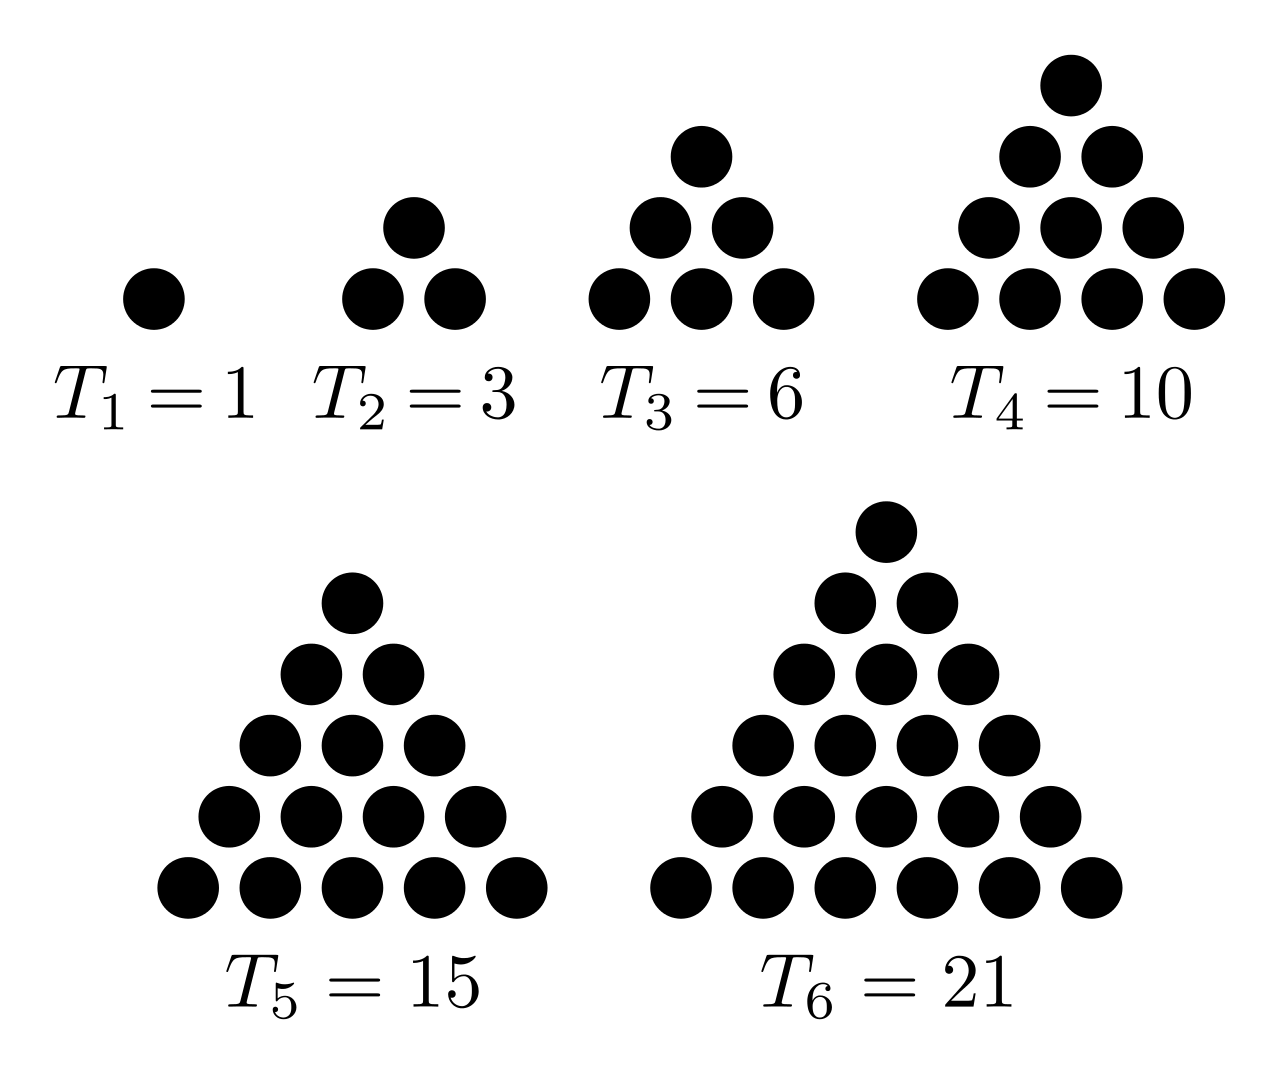
\includegraphics[scale=0.10]{triangular_numbers.png}
 \columnbreak
 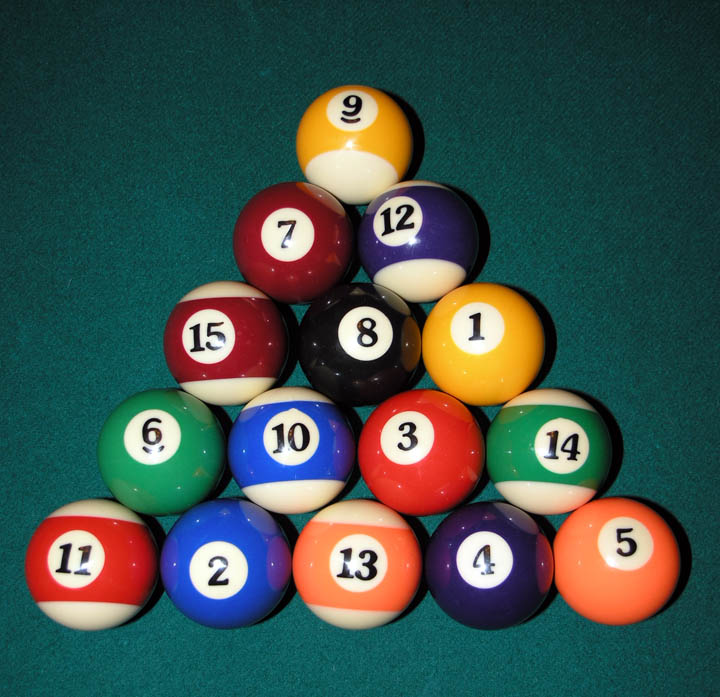
\includegraphics[scale=0.15]{pool.jpg}
 \end{multicols}
\end{center}
\end{frame}

\begin{frame}
\frametitle{Heavy digression: Handshake problem}
{
\definecolor{amber}{rgb}{1.0, 0.75, 0.0}
\setbeamercolor{block title}{bg=amber}
\begin{block}{Problem}

In a room of $n$ people, how many ways are there for them to shake hands without shaking the same hand twice?
\end{block}

\begin{block}{Solution}
Big surprise, the answer is triangular numbers (specifically $T_{n+1}$ in this case)
\end{block}
}

\vspace{2em} 

How would we do this in C++20?
\end{frame}

\begin{frame}
\frametitle{Last digression: flashback to 8th grade}
Rather than computing solutions directly, we can check if a number is a solution by seeing if it is a triangular number.

\begin{equation}\tag{Formula for finding triangular numbers}
T_n = \frac{n(n+1)}{2}
\end{equation}

\begin{equation}\tag{Inverse of the formula above}
n = \frac{\sqrt{8T_n + 1} - 1}{2}
\end{equation}

\vspace{2em}

Result: For any integer $x$, if $8x+1$ is a perfect square, then $x$ is a solution to our problem.

\end{frame}

\begin{frame}[fragile]
\frametitle{Range comprehensions}
Our official solution to this problem looks like this.

\lstset{language=C++,
		numbers=left,
		stepnumber=1,
		firstnumber=1,
		xleftmargin=2em,
		frame=single,
		framexleftmargin=2em,
		numberfirstline=true,
		breakatwhitespace=true,
                basicstyle=\fontsize{8}{9}\ttfamily,
                keywordstyle=\color{blue}\ttfamily,
                stringstyle=\color{red}\ttfamily,
                commentstyle=\color{green}\ttfamily,
                morecomment=[l][\color{magenta}]{\#}
}
\begin{lstlisting}
    #include <ranges>
    #include <cmath>
    
    using namespace std;    
    
    auto solution = ranges::view::ints(1) | 
    ranges::view::for_each([](int i)
    {
    
    return yield_if( sqrt(8*i + 1) * sqrt(8*i + 1) == 8*i + 1); 
    
    });
    // print the first 100 solutions
    ranges::for_each(solution | 
    view::take_while([](int i){ return i < 100; }), [](int i)
    {
         cout << i << endl;
    });
\end{lstlisting}
\end{frame}

\begin{frame}
\frametitle{Range comprehension in-depth}
\begin{itemize}
\setlength\itemsep{2em}
\item Range comprehensions are analogous to function composition, but can be more terse (this is either a good thing or a bad thing)
\item Again, we used lazy evaluation
\item The yield statement was an example of a generator, which is a special case of coroutines

\item Note: Commitee is still considering adding support for coroutines
\end{itemize}
\end{frame}

\section{Contracts}
\begin{frame}
\frametitle{Contracts}
Some basic review:
\begin{itemize}
\item Preconditions: " a predicate that is supposed to hold upon entry in a function"
\item Postconditions: " a predicate that is supposed to hold upon exit from the function"
\end{itemize}

\vspace{2em}
Saying that Contracts are like \texttt{assert()} on steroids is a major understatement
\end{frame}

\begin{frame}[fragile]
\frametitle{Simplest example: Queues}

\lstset{language=C++,
		numbers=left,
		stepnumber=1,
		firstnumber=1,
		xleftmargin=2em,
		frame=single,
		framexleftmargin=2em,
		numberfirstline=true,
		breakatwhitespace=true,
                basicstyle=\fontsize{8}{9}\ttfamily,
                keywordstyle=\color{blue}\ttfamily,
                stringstyle=\color{red}\ttfamily,
                commentstyle=\color{green}\ttfamily,
                morecomment=[l][\color{magenta}]{\#}
}
\begin{lstlisting}
    auto push(Queue& queue, int value)
    [[ expects: queue.full() == false ]]
    [[ ensures: queue.empty() == false ]]
    {
     // code goes here
     [[ assert: queue.is_ok() ]]
    }
\end{lstlisting}

\begin{itemize}
\item Surprisingly, this is pretty self-explanatory
\end{itemize}

\end{frame}

% https://www.arcos.inf.uc3m.es/jdgarcia/wp-content/uploads/sites/9/2017/04/contracts.pdf
\begin{frame}
\frametitle{Contracts: in-depth}
The syntax  is \\ \texttt{[[ contract-attribute modifier: conditional expression ]]}

\begin{itemize}
\setlength\itemsep{2em}
\item \texttt{contract-attribute}:  This is one of \textit{expects}, \textit{ensures} , \textit{assert}
\item \texttt{modifier}: Possible values are 
\begin{enumerate}
\item \texttt{default}
\item \texttt{audit}
\item \texttt{axiom}
\end{enumerate}

\end{itemize}
\vspace{2em}
The hype around Contracts is that \emph{you} get to choose what each of those modifier levels means \textbf{and} what happens when your contract is violated

\end{frame}

\begin{frame}
\frametitle{"Build levels"}

This is a compiler-specified option that determines \textit{what contracts will be checked}.

\begin{itemize}
\item \texttt{off} : No contracts whatsoever are run.

\item \texttt{default} : Only contracts with the \texttt{default} level are checked

\item \texttt{audit} : Contracts with the \texttt{audit} and \texttt{default} levels are checked
\end{itemize}

\vspace{2em}
You {\Large{cannot}} change the build level in source code

\end{frame}


\begin{frame}[fragile]
\frametitle{So what if I violate the contract?}

\textcolor{red}{By default, failing contracts mean program termination}
\vspace{1em}
\begin{itemize}
\setlength\itemsep{1.5em}
\item However, there are \textbf{contract violation handlers}

\item As the name implies, this is the function that gets called when a contract is violated

\item There is one contract violation handler per \textit{translation unit} (output of pre-processor)

Must have specific signature:

\lstset{language=C++,
		xleftmargin=2em,
		frame=single,
		framexleftmargin=2em,
		numberfirstline=true,
		breakatwhitespace=true,
                basicstyle=\fontsize{8}{9}\ttfamily,
                keywordstyle=\color{blue}\ttfamily,
                stringstyle=\color{red}\ttfamily,
                commentstyle=\color{green}\ttfamily,
                morecomment=[l][\color{magenta}]{\#}
}
\begin{lstlisting}
    void(const std::contract_violation &);
\end{lstlisting}

\end{itemize}
\end{frame}

\begin{frame}
\frametitle{So is that it?}

If only...

\vspace{2em}

\begin{itemize}
\setlength\itemsep{2em}
\item After the contract violation handler is reached, there's two options:
\begin{enumerate}
\item Program terminates indefinitely (default option is none is specified!)
\item Program continues
\end{enumerate}

\item This option is called the \emph{continuation mode} and can only be set through the compiler (not source code)

\item You cannot determine the current continuation mode inside of source code
\end{itemize}
\end{frame}

\begin{frame}
\frametitle{Contracts: Benefits}

How does this compare to the regular \texttt{assert()} macro?
\begin{itemize}
\setlength\itemsep{2em}
\item This isn't a macro

\item You can handle custom behavior on violations

\item Contracts enable compilers to perform more optimizations

\item With \texttt{assert()} only, its hard to impose precondition checks because you may not always have access to calling site of a function
\end{itemize}
\vspace{1em}

Herb Sutter (chair of the C++ Committee) has personally said he thinks \textit{"contracts is the most impactful feature of C++20 so far"}


\end{frame}

%----------------------------------------------------------------------------------------

\section{Atomic shared pointers}

\begin{frame}
\frametitle{Atomic shared pointers}

\begin{itemize}
\setlength\itemsep{2em}
\item Nothing to do with chemistry

\item .. Despite being the "A" in \textit{ACID}
\item "Aren't smart pointers already thread-safe?"

\end{itemize}
\end{frame}


\begin{frame}
\frametitle{The answer is: kind of?}
Here's how smart pointers are implemented

\vspace{1em}
\begin{center}
\includegraphics[scale=1]{smart_pointers.png}
\end{center}
\begin{itemize}
\item The control block is thread-safe 
\item Access to the object \emph{isn't}
\end{itemize}
\end{frame}

\begin{frame}[fragile]
\frametitle{Wanna race?}

\lstset{language=C++,
		numbers=left,
		stepnumber=1,
		firstnumber=1,
		xleftmargin=2em,
		frame=single,
		framexleftmargin=2em,
		numberfirstline=true,
		breakatwhitespace=true,
                basicstyle=\fontsize{8}{9}\ttfamily,
                keywordstyle=\color{blue}\ttfamily,
                stringstyle=\color{red}\ttfamily,
                commentstyle=\color{green}\ttfamily,
                morecomment=[l][\color{magenta}]{\#}
}
\begin{lstlisting}
    std::shared_ptr<int> pointer  = std::make_shared<int>(2011);
    
    for (auto i = 0; i < 10; i++)
    {
    	std::thread([&pointer]
    	{
    		pointer = std::make_shared<int>(2014);
    	}).detach();
    
    }
\end{lstlisting}

I can't take credit for this example, but it illustrates the point...

\end{frame}

\begin{frame}
\frametitle{To be fair...}
\begin{itemize}
\setlength\itemsep{2em}
\item There technically are atomic operations you can do on shared pointers
\item \texttt{std::atomic\_is\_lock\_free}, \texttt{std::atomic\_exchange}, a handful of others
\item Like with many things in C++, the right usage of these takes discipline
\item ... which make it error-prone
\item Atomic pointers are going to solve this
\end{itemize}
\end{frame}

\begin{frame}[fragile]
\frametitle{Don't believe me?}

\begin{multicols}{2}
\lstset{language=C++,
		numbers=left,
		stepnumber=1,
		firstnumber=1,
		xleftmargin=2em,
		frame=single,
		framexleftmargin=2.5em,
		numberfirstline=true,
		breaklines=true,
                basicstyle=\fontsize{6}{7}\ttfamily,
                keywordstyle=\color{blue}\ttfamily,
                stringstyle=\color{red}\ttfamily,
                commentstyle=\color{green}\ttfamily,
                morecomment=[l][\color{magenta}]{\#}
}
\begin{lstlisting}
 template<typename Type> class concurrent_stack {
    struct Node { Type t; shared_ptr<Node> next; };
    atomic_shared_ptr<Node> head;
    concurrent_stack( concurrent_stack &) =delete;
    void operator=(concurrent_stack&) =delete;
    
    public:
    concurrent_stack() =default;
    ~concurrent_stack() =default;
    class reference {
        shared_ptr<Node> p;
    public:
       reference(shared_ptr<Node> p_) : p{p_} { }
       Type& operator* () { return p->t; }
       Type* operator->() { return &p->t; }
    };
    
    auto find(Type t) const {
        auto p = head.load();  
        while( p && p->t != t )
            p = p->next;
        return reference(move(p));
    }
    auto front() const {
       return reference(head); 
    }
    void push_front(Type t) {
      auto p = make_shared<Node>();
      p->t = t;
      p->next = head;         
      while( !head.compare_exchange_weak(p->next, p) ){ }
    }
    void pop_front() {
       auto p = head.load();
       while( p && !head.compare_exchange_weak(p, p->next) ){ }
    }
};

\end{lstlisting}
\columnbreak
\end{multicols}
\end{frame}

\begin{frame}
\frametitle{Told you}

That last slide:

\begin{itemize}
\setlength\itemsep{2em}
\item was a 
\textbf{40-line} implementation of a \emph{thread-safe}, (singly) linked list
\item The word "atomic" only showed up once
\item You could have written thread-safe code without knowing what a thread was
\item In C++17, you'd have had to use the atomic member functions every time you touched the head pointer
\end{itemize}

\end{frame}

\section{Miscellaneous}

\begin{frame}
\frametitle{Any sci-fi fans out there?}
\begin{itemize}
\setlength\itemsep{2em}
\item C++20 adds a three-way comparison operator (\texttt{<=>})
\item Sometimes people call this the spaceship operator
\item Given two values $A$ and $B$, this operator checks each of the following
\begin{enumerate}
\item Is $A < B$ ?
\item Is $A = B$ ?
\item Is $A > B$ ?
\end{enumerate}

\item Perl, Haskell and Ruby, have this

\item This is an extension of C's \texttt{strcmp()}
\end{itemize}
\end{frame}

\begin{frame}
\frametitle{Wrapping up..}

\begin{itemize}
\setlength\itemsep{1.5em}
\item "Concepts" : essentially type-checking for templates
\item Ranges: Big step up from existing iterators approached introduced in C++11
\item Contracts: Basically keeps your code in check; depending on how this is fully implemented it could end up being a huge pain or very convenient
\item Atomic smart pointers: Thread safety meets smart pointers, you may not use this often but when you do you'll be thankful
\item Threeway-comparison operator: \texttt{strcmp()} all the things
\end{itemize}
\end{frame}

\begin{frame}
\frametitle{Conclusion / going forward}
\begin{itemize}
\setlength\itemsep{1.5em}
\item Overall I personally think the new additions will be pretty useful, others may see it as bloat
\item As a beginner, I appreciate that these changes make the language a bit more noob-friendly
\item C++20 might not as game-changing as the C++11 standard, but its still fairly significant
\item Now is probably a good time to start thinking about how we can port our codebase over to C++20 when it arrives ?
\item Round 2 of presentation, December 2019 -- discussing what features have been deprecated/removed?
\end{itemize}
\end{frame}

\begin{frame}
\Huge{\centerline{The End}}
\end{frame}

\end{document} 